\documentclass[12pt]{article}
\usepackage[spanish]{babel}
\usepackage{natbib}
\usepackage{url}
\usepackage{float}
\usepackage[utf8]{inputenc}
\usepackage{amsmath}
\usepackage{graphicx}
\usepackage{fancyhdr}
\usepackage{vmargin}
\usepackage{listings}
\usepackage{hyperref}
\setmarginsrb{3 cm}{2.5 cm}{3 cm}{2.5 cm}{1 cm}{1.5 cm}{1 cm}{1.5 cm}

\title{Tarea - 01}
\date{\today}

\makeatletter
\let\thetitle\@title
\let\theauthor\@author
\let\thedate\@date
\makeatother

\pagestyle{fancy}
\fancyhf{}
\rhead{\theauthor}
\lhead{\thetitle}
\cfoot{\thepage}

\addto\captionsspanish{
  \renewcommand{\contentsname}%
    {Tabla de contenido}%
}

\begin{document}
    \pagestyle{fancy}
    \fancyhf{}

    \lhead{\begin{picture}(0,0) \put(0,0){
\includegraphics[width=30mm]{images/Logo2.png}} \end{picture}}
    \renewcommand{\headrulewidth}{0.7pt}
    \fancyhead[R]{Procesamiento de lenguaje natural - Tarea 01}
\fancyfoot[R]{\thepage}

\begin{titlepage}
	\centering
    
\includegraphics[scale = 0.45]{images/Logo.png}\\[0.5 cm]	% University Logo
    \textsc{\large Universidad de los Andes\\
        \vspace{0.2cm} 
        Facultad de ingeniería\\
        \vspace{0.3cm} 
        Tarea 01}\\[2.0 cm]	% University Name
	\textsc{\Large Procesamiento de lenguaje natural}\\[0.5 cm]
	% Course Code
	\rule{\linewidth}{0.2 mm} \\[0.4 cm]
	{ \LARGE \bfseries \thetitle}\\
	\rule{\linewidth}{0.2 mm} \\[1.5 cm]
	
	\large
			\emph{Presentado por:} \\
			Juan David García Hernández\\
			Nicolás Rocha Pacheco\\
			César Daniel Garrido Urbano\\
	\vfill
	\large
			\emph{Presentado a:}\\
			Rubén Francisco Manrique Pirmanrique\\
\end{titlepage}

\thispagestyle{empty}
\tableofcontents
\pagebreak

\setcounter{page}{1}
\section*{Introducción}
De acuerdo con \cite{IR-book} Recuperación de Información o IR por sus siglas en inglés hace referencia a la encontrar material que satisfaga una necesidad de información. Usualmente, este material son documentos de texto y se almacena en computadores. Hasta hace algunos años esta actividad se limitaba a algunas profesiones específicas. No obstante, el \textit{boom} del internet ha ocasionado que la mayoría de estas búsquedas se hagan a través de este, sea mediante motores de búsqueda o correo electrónico.\\

Para IR se han propuesto diferentes métodos que permiten solucionar el problema desde diferentes ángulos. A continuación, se explica la implementación de técnicas 4 diferentes técnicas y se comparan sus resultados.
\section{Métricas de evaluación para Recuperación de Información}
Antes de realizar una implementación de un sistema de búsqueda de información es necesario definir métricas de evaluación. Las métricas de evaluación van a permitir comparar cuantitativamente los diferentes sistemas e implementaciones. A lo largo de este documento se usarán siete métricas diferentes: precisión, precisión en K, recall en K, precisión-promedio, MAP, DCG y NDCG. A lo largo de esta sección se introducen las métricas, su interpretación y la metodología usada para su cálculo. 

\subsection{Precisión}
La precisión es una métrica que permite evaluar qué porcentaje del resultado de una consulta es relevante para la búsqueda. Teniendo en cuenta que en el problema de la búsqueda de información retorna conjuntos de elementos discretos, la precisión ($P$) se puede definir como se presenta en la ecuación (\ref{eq:precision}). En dicha ecuación se evalúa la cardinalidad de la intersección del conjunto de elementos retornados por el sistema de búsqueda de información y el conjunto de los documentos que efectivamente son relevantes a la búsqueda. Este valor es normalizado a partir de la cardinalidad del conjunto de documentos retornados.

\begin{equation}
    P = \frac{|RET \cap REL|}{|RET|}
    \label{eq:precision}
\end{equation}

\subsection{Precisión en K}
Una alternativa de la precisión es evaluarla sobre un subconjunto de los documentos relevantes y los documentos recuperados. Al aplicar esta métrica lo que se hace es evaluar la precisión considerando una cantidad determinada de documentos. La cantidad de documentos suele ser denominada con la letra $K$. Esta métrica suele ser usada en conjuntos de datos donde no es factible conocer el conjunto de documentos relevantes en su totalidad. La ecuación X presenta cómo se calcula esta métrica.

\begin{equation}
    P@K = \frac{|RET \cap REL|}{K}
\end{equation}

\subsection{Recall en K}
El recall 

\subsection{Precisión-Promedio}

\subsection{MAP}

\subsection{DCG}

\subsection{NDCG}

\section{Estrategias de recuperación de información}
 A continuación, se explica la implementación de cuatro técnicas diferentes y se comparan sus resultados.
\subsection{Búsqueda binaria (BS)}
La búsqueda binaria es un algoritmo en que se utilizan operaciones lógicas como AND y OR con el fin de encontrar documentos que contienen los términos solicitados en la consulta, asumiendo que ello indica que son relevantes para dicha necesidad de información. Para llevar a cabo la búsqueda de manera eficiente, se crea una matriz binaria indicando los términos que contiene cada documento, dando a la técnica el nombre de \textit{búsqueda binaria}. A continuación, se explica detalladamente el proceso que sigue la técnica.

\subsubsection{Funcionamiento de BS}
Una vez se conoce de cada documento los términos que contiene y su frecuencia, se procede a construir la matriz binaria. Las filas de esta matriz corresponden a los documentos que se consideran en la búsqueda y las filas corresponden a los términos existentes en el diccionario. Siendo así, los registros de cada columna que corresponden a uno indican que ese término existe en el documento indicado por la columna. Cabe resaltar que la frecuencia no es considerada en esta técnica. En la figura \ref{fig:b_matrix} se muestra un ejemplo de cómo se vería una matriz binaria.\\

\begin{figure}[H]
    \centering
    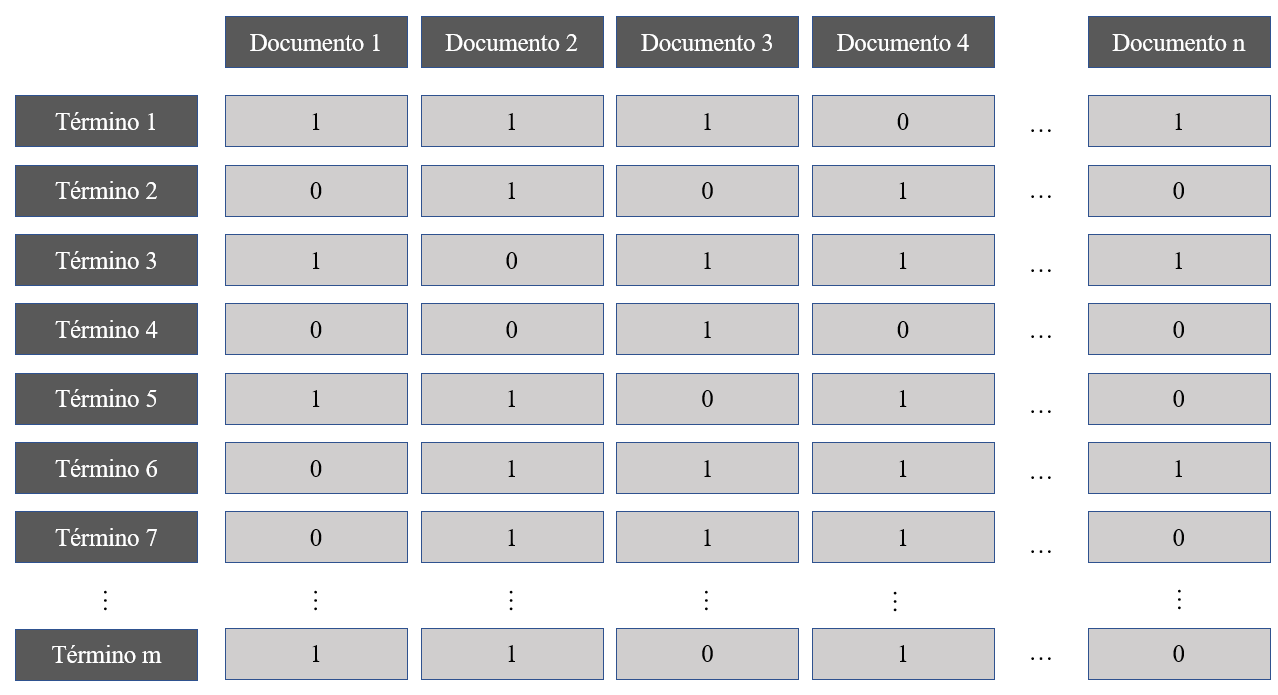
\includegraphics[scale=0.5]{doc/images/BS/b_matrix.PNG}
    \caption{Matriz binaria ejemplo}
    \label{fig:b_matrix}
\end{figure}

Tras recibir la consulta (palabras claves que caracterizan la necesidad de información) se procede a construir un vector del tamaño del vocabulario que indica, al igual que la matriz, qué términos incluye la consulta, generando así un vector binario disperso. En la figura \ref{fig:b_query} se muestra cómo sería el vector de la consulta.\\

\begin{figure}[]
    \centering
    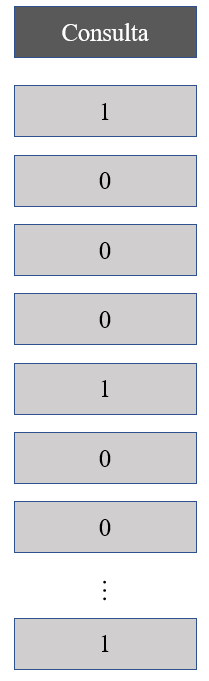
\includegraphics[scale = 0.5]{doc/images/BS/b_query.PNG}
    \caption{Vector binario de la consulta}
    \label{fig:b_query}
\end{figure}

En el caso específico del \textit{dataset} trabajado la matriz tiene dimensión de 17.365 filas, 331 columnas, dado que se tiene un vocabulario de 17.365 términos.\\

Con el fin de almacenar de manera eficiente una matriz de tamaño (5'747.815) se procede a utilizar el tipo de dato que menor espacio de memoria ocupa. Al momento de crear la matriz se indica el tipo de dato a utilizar, el cual corresponde a \url{numpy.bool\_}. Para guardar y abrir la matriz se utilizan las funciones estándar de numpy (\url{load} y \url{save}).\\

Ahora bien, una vez se tiene el vector que representa la consulta y la matriz que almacena toda la información de términos por documento, se utiliza una operación lógica que permita seleccionar los documentos que contienen uno o todos los términos consultados. En el primer caso se utiliza la operación lógica OR, lo cual indica que se extraerán los documentos que tienen al menos uno de los términos buscados; en caso contrario, se utiliza AND para obtener los documentos que tienen todos y cada uno de los términos buscados.\\

Como es de esperarse es poco común que un documento contenga exactamente todos los términos al igual que es muy probable que algún documento tenga al menos uno de los términos, ocasionando el fenómeno conocido como \textit{feast and famine}. Este indica que las consultas binarias tienen la desventaja de devolver muy pocos o ningún documento (\textit{famine}) en el caso de AND o devolver demasiados documentos (\textit{feast}) al usar OR.

\subsubsection{Explicación de la implementación}
En el \textit{notebook} \url{HW01_2.ipynb} se presenta la implementación de la técnica descrita previamente.\\

En primer lugar se procede con la construcción de la matriz. Para ello, después de importar los \textit{corpus} tanto de vocabulario como de consultas, se recorre cada uno de los documentos insertando un '1' en los registros correspondientes de la matriz. Dichos registros son las coordenadas de la matriz en donde el número de documento corresponde al que se está recorriendo y el término a aquel encontrado en el documento.\\

Posteriormente, se realiza un proceso similar para la vectorización de la consulta. Se crea un vector, igualmente binario, del tamaño del vocabulario. En este vector se almacenan unos en cada uno de los términos que aparece en la consulta hecha.\\

Teniendo esta matriz y el vector de consulta se procede a multiplicar por elemento cada vector columna de la matriz, correspondiente a un documento, con el vector asociado a la consulta. El resultado tendrá '1' en todos aquellos términos que aparezcan tanto en la consulta como en el documento. Es en este punto en donde aplica la operación lógica AND u OR. Si la operación utilizada es conjunción el documento será retornado como relevante en caso de que contenga todas y cada una de las palabras de la consulta. Por otra parte, en caso de que se utilice la disyunción, todos los documentos que contengan uno o más de los términos. En el caso de la operación OR se utiliza la función \url{any}, en el primer caso con el fin de saber si algún término de los buscados está en el documento. En el caso de la operación AND se revisa que el total de términos encontrados sea igual al total buscados.\\

La función previamente descrita retorna una lista con los índices de documentos considerados como relevantes. Finalmente, se recorre todo el listado de consultas y se almacenan todos los documentos devueltos por la función para cada consulta. Los resultados obtenidos se analizarán en la sección correspondiente.

\subsection{Búsqueda binaria usando índice invertido (BSII)}
La búsqueda binaria con índice invertido (BSII, \textit{Binary Search with Inverted Index}) es una evolución de la búsqueda binaria presentada previamente. Como su nombre lo indica, esta aproximación al problema de búsqueda de información utiliza un índice invertido: una estructura de datos donde se relaciona cada término del vocabulario con los documentos donde está presente. En este sentido, cada término va a estar vinculado con lo que se conoce como una lista de posteo (\textit{posting list}) donde cada ítem de dicha lista es el identificador de un documento donde aparece el término. Con el fin de optimizar el proceso de recuperación de la información se suele incluir la frecuencia relativa de cada término dentro del índice invertido. La figura \ref{fig:inverted_index} presenta una representación de un índice invertido, donde se pueden evidenciar los términos, la frecuencia relativa y la lista de posteo.

\begin{figure}[ht]
    \centering
    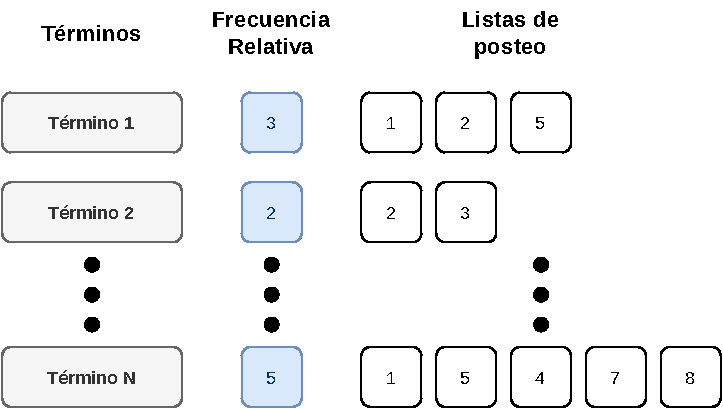
\includegraphics[width=0.7\textwidth]{images/BSII/II.pdf}
    \caption{Representación de un índice invertido. Se puede evidenciar una serie de términos al cual se asocia su frecuencia relativa y una lista de posteo con los identificadores de los documentos donde aparecen.}
    \label{fig:inverted_index}
\end{figure}

\subsubsection{Construcción del Índice Invertido}
Según \cite{IR-book} existen cuatro estrategias principales para construir eficientemente un índice invertido de búsqueda binaria (BSII, \textit{Binary Search Inverted Index}. La selección de una es estas estrategias depende de las características del hardware sobre el cuál vaya a ser implementada, especialmente en lo que se refiere al número de máquinas que van a ejecutar el algoritmo. 

Vale la pena mencionar que algunos de los valores presentados en \cite{IR-book} incluyen valores y consideraciones propias de sistemas típicos de 2007. Es necesario tener en cuenta que desde 2007 hasta la actualidad (2021) se han presentado avances de hardware que pueden afectar los algoritmos de construcción del índice invertido y búsqueda de información.

Las estrategias para construir el índice invertido son: indexado basado en ordenamiento en bloques (BSBI, \textit{Blocked Sort-Based Indexing}), indexado en memoria de un solo paso (SPIMI, \textit{Single-Pass In-Memory Indexing}), indexado distribuido e indexado dinámico. Tanto el BSBI como el SPIMI están contemplados como estrategias para ser usadas en una máquina, mientras que el indexado distribuido y el indexado dinámico suelen ser usados en grupos de máquinas. 

Dado que la solución del enunciado debe ser realizada exclusivamente en una máquina, debido al tamaño de la base de datos y la disponibilidad de recursos, solo serán revisadas las estrategias de BSBI y SPIMI. Las dos estrategias están contempladas para realizar un único paso por los datos para construir el índice.

\paragraph{Indexado Basado en Ordenamiento en Bloques (BSBI)} Esta estrategia es utilizada para construir el índice invertido dividiendo la colección en bloques de igual tamaño que son analizadas en memoria. Para cada bloque se realiza el siguiente proceso:

\begin{enumerate}
    \item Se recupera el siguiente bloque de la colección.
    \item El bloque es procesado para extraer parejas de identificador del término e identificador del documento (\textit{termID} - \textit{docID}).
    \item Se invierten el bloque para construir un resultado intermedio del índice invertido. El resultado de este proceso es que para un identificador de un término se tendrá una lista con los identificadores de los documentos en los que aparece.
    \item Los resultados intermedios para cada bloque son almacenados temporalmente en el almacenamiento secundario.
    \item Una vez se han invertido todos los bloques de la colección, los resultados intermedios se unen en lo que será el índice invertido.
\end{enumerate}

La idea de dividir la colección en bloques de igual tamaño tiene el propósito de realizar lecturas contiguas en el almacenamiento secundario. De esta manera, los tiempos de lectura son inferiores a lo que sería una serie lecturas aleatorias en el disco.

Un factor crítico de esta estrategia es el procesamiento del texto para la extracción de las parejas de identificadores de términos y documentos. La estructura de datos que realiza la relación entre término y su identificador podría llegar a ocupar una gran cantidad de espacio de memoria para colecciones lo suficientemente grandes. Esta situación se corrige con la estrategia SPIMI. 

\paragraph{Indexado en Memoria de un Solo Paso (SPIMI)}
La estrategia SPIMI busca construir el índice invertido a partir de los términos directamente. El objetivo de SPIMI consiste en crear un diccionario de forma dinámica conforme se van leyendo las parejas de término e identificador del documento. De forma general, el algoritmo de SPIMI realiza el siguiente proceso:

\begin{enumerate}
    \item Se crea un archivo de salida y un diccionario. El archivo de salida será usado para almacenar los resultados intermedios. En este caso, el resultado intermedio será el diccionario.
    \item Se va iterando sobre cada pareja de término e identificador del documento. Si el término está en el diccionario, se recupera la su entrada y se agrega el nuevo identificador de documento. Se lo contrario, se agrega la entrada en el documento. 
    \item Cuando la memoria se llena, se organizan los términos del diccionario con un orden lexicográfico y se escriben en el almacenamiento secundario.
    \item Una vez se han procesado todas las parejas, se realiza la unión de los diccionarios para obtener el índice invertido.
\end{enumerate}

Una de las ganancias que se obtiene al utilizar la estrategia SPIMI en comparación al BSBI es que no es necesario ordenar las parejas de términos e identificadores de documentos durante la construcción del índice. Otro beneficio consiste en que, como se indicó previamente, SPIMI no requiere de una estructura de datos que asocie un término con su identificador, por lo que la memoria principal puede ser usada eficientemente.

\subsubsection{Gestión de Recursos y Acceso a Memoria}
Dado que un índice invertido puede ser una estructura que ocupe una gran cantidad de espacio de almacenamiento, es necesario establecer estrategias con el fin de que dicha estructura sea accesible de forma eficiente y que requiera menos almacenamiento. En primer lugar, es necesario prevenir que el índice va a ser guardado en el almacenamiento secundario ya que es probable que ocupe más espacio del provisto por la memoria principal. En este orden de ideas deben solucionarse dos situaciones: el índice debe ser accedido en el almacenamiento secundario de forma rápida y debe ocupar el menor espacio posible.

Para disminuir el tiempo de acceso al índice es posible hacer uso de la jerarquía de memoria y el principio de localidad para cachear (\textit{caching}) las listas de posteo en la memoria principal. De esta manera se reduce el tiempo de acceso al índice para los términos que se usan con mayor frecuencia. Por otra parte, se pueden utilizar algoritmos de compresión y descompresión con el fin de disminuir el espacio de almacenamiento requerido para el índice. El uso de dichos algoritmos tiene dos beneficios: reduce el espacio utilizado en el almacenamiento secundario y permite incluir más términos en la memoria principal.

Es necesario considerar que un índice está compuesto por el vocabulario y las listas de posteo, donde el primero ocupa un espacio de almacenamiento considerablemente menor al segundo. En este contexto, es necesario establecer estrategias diferentes de compresión dependiendo de si el elemento a comprimir es el vocabulario o las listas de posteo. Para comprimir el diccionario se pude recurrir a codificarlo como una cadena de caracteres donde se incluya el término, su frecuencia relativa y un puntero a su lista de posteo. Esta estrategia de compresión puede se complementada con un agrupamiento de los términos en bloques de un tamaño definido. Al implementar estas dos estrategias de compresión es posible reducir la cantidad de almacenamiento requerido por el diccionario. Sin embargo, el tiempo de acceso para este puede verse afectado, especialmente al implementar el agrupamiento. 

El caso de las listas de posteo tiene mayor incidencia en el tamaño del diccionario dado que corresponden a la mayor parte de los datos que deben ser almacenados. En primer lugar, es necesario tener en cuenta que las listas de posteo se pueden definir como el identificador de un documento inicial y una serie de incrementos relativos a este. En este sentido, es posible codificar dichos incrementos como una serie de valores de tamaño dinámico en contraposición a valores de tamaño fijo. De esta manera se puede garantizar que el almacenamiento empleado para codificar los incrementos sean usados eficientemente. Existen dos estrategias para codificar dichos incrementos de forma dinámica: codificar a nivel de bytes y a nivel de bits. 

\subsubsection{Solución de Consultas al Índice Invertido}
Una consulta al índice invertido permite realizar búsquedas binarias usando los operadores lógicos AND, OR y NOT. Por una parte se tiene que dos términos con conjuntivos si se relacionan mediante un operador AND y disjuntos si se relacionan con un operador OR. Con el fin de resolver una consulta al índice invertido es necesario recuperar las listas de posteo de los dos términos y realizar la intersección de las dos listas según el operador lógico usado. Naturalmente, en caso que algún término sea modificado mediante el operador NOT, es necesario establecer el complemento de la lista de posteo de dicho término. Una vez se ha realizado la intersección de las dos listas se puede retornar el resultado o continuar con los demás términos de la consulta.

Un aspecto clave de la consulta a un índice invertido es la intersección entre dos listas de posteo. En [1] se presenta un algoritmo de intersección para dos listas de posteo con un operador de conjunción (AND). Sin embargo, este debe modificarse para que pueda incluir una intersección disjunta (OR) y un operador de modificación (NOT). El listado \ref{lst:intersect} presenta el algoritmo para realizar la intersección de dos listas de posteo con operadores conjuntivos, disjuntos y de modificación.

\begin{lstlisting}[
    basicstyle=\scriptsize,
    caption={Algoritmo para la intersección de listas de posteo con operadores conjuntivos, disjuntos y de modificación.}, 
    label=lst:intersect, 
    captionpos=b,
    abovecaptionskip=1em,
    belowcaptionskip=1em
]
INTERSECT(p1, p2, op, mod1, mod2, n):
    if mod1 == NOT do
        p1 = complement(p1, n)
    
    if mod2 == NOT do
        p2 = complement(p2, n)
        
    if length(p2) < length(p1) do
        p1, p2 = p2, p1
        
    answers = []
    indexes = [0, 0]
    finish = false
    
    while not finish do
        posting1 = p1[indexes[0]]
        posting2 = p2[indexes[1]]
    
        if operator == AND do
            if posting1 == posting2 do
                append(answers, posting1)
                
            if posting1 < posting2 do
                increment(indexes[0])
            else do
                increment(indexes[0])
                
            if indexes[0] == length(p1) and indexes[1] == length(p2) do
                finish = true
        
        else do
            if indexes[0] != length(p1) do
                if posting1 < posting2 do
                    append(answers, posting1)
                    increment(indexes[0])
                
                else if posting1 == posting2 do
                    append(answers, posting1)
                    increment(indexes[0])
                    increment(indexes[1])
                    
                else do
                    append(answers, posting2)
                    increment(indexes[1])
                    
            else do
                append(answers, posting2)
                increment(indexes[1])
                
            if indexes[1] == length(p2) do
                finish = true
        
\end{lstlisting}

En la ejecución del algoritmo presentado en el listado \ref{lst:intersect} se realizan los siguientes pasos:

\begin{itemize}
    \item Se realiza la modificación (\texttt{mod1}, \texttt{mod2}) de las listas de posteo (\texttt{p1} y \texttt{p2}) dependiendo del número de documentos presentes en la colección (\texttt{n}). Se asume que los identificadores de los documentos hacen parte de un conjunto de enteros que van desde el número uno hasta \texttt{n}.
    \item Se organizan las listas de posteo de modo tal que \texttt{p1} apunte a la lista de menor tamaño y \texttt{p2} apunte a la lista de mayor tamaño.
    \item Se crea un arreglo vacío para almacenar las respuestas y otro con dos enteros que almacenan los índices para las listas de posteo.
    \item Se itera mientras que no se haya alcanzado la condición de parada. En primer lugar se recuperan los elementos de las listas de posteo según los índices almacenados en el arreglo correspondiente. Dependiendo del operador (\texttt{op}) se realizan las siguientes acciones dentro del ciclo:
    
    \begin{itemize}
        \item Si se trata de una intersección conjuntiva se revisa si los dos elementos son iguales. En caso que sean iguales se agregan al arreglo de respuestas. Se incrementa el índice del elemento que corresponda al menor valor. Cuando los dos índices alcancen la longitud de la lista se activa la condición de parada.
        \item Si se trata de una intersección disjunta se revisa si el primer índice no haya alcanzado la longitud de la primera lista de posteo. Si el elemento de la primera lista es inferior al elemento de la segunda, el primer elemento es agregado al arreglo de respuestas y el índice de la primera lista incrementado. En caso tal que los dos elementos sean iguales, uno de estos se agrega a la lista de respuestas y los dos índices se incrementan. Finalmente, si el elemento de la segunda lista es mayor, este es agregado a las respuestas y su índice es aumentado. En caso tal que el primer índice haya alcanzado la longitud de su lista correspondiente, se agregan los elementos restantes de la segunda lista al arreglo de respuestas. Cuando se han agregado todos los elementos de la segunda lista se agrega la condición de parada.
    \end{itemize}
\end{itemize}

Si una consulta contiene más de dos términos es necesario establecer una estrategia para optimizar la recuperación de las listas de posteo y su intersección. Una de las estrategias con mayor adopción consiste en organizar la intersección de las listas según la frecuencia relativa de los términos. No obstante, esta estrategia de implementación es válida para las intersecciones conjuntivas. Es necesario modificar la estrategia levemente con el fin de incluir tanto las operaciones disjuntas. En este orden de ideas, una estrategia sería resolver las operaciones disjuntas en orden incremental antes de resolver las operaciones disjuntas.


\subsubsection{Implementación}
Teniendo en cuenta que la implementación se haría en Python y que esta sería ejecutada en una máquina, se podría partir de la estrategia SPIMI para construir el índice invertido. Esta decisión se toma en base a las siguientes consideraciones:

\begin{itemize}
    \item SPIMI no requiere un mayor control sobre la memoria principal como sí lo requiere BSBI. Dado que Python no ofrece métodos para realizar este control, dado que es un lenguaje de alto nivel, se favorece la implementación de SPIMI sobre BSBI.
    \item Python ofrece diccionarios de forma nativa. Estos diccionarios pueden contener como llave (\textit{key}) la cadena de texto del término en cuestión y como valor (\textit{value}) una lista con los identificadores del documento.
    \item Con la implementación de listas nativas de Python no es necesario alocar memoria directamente desde el algoritmo. Python hace esto sin que el programador deba indicarlo explícitamente.
\end{itemize}

Aprovechando dicha estrategia se tiene que el conjunto de datos es almacenado enteramente en la memoria, por lo que no es necesario implementar una estrategia de lectura en el almacenamiento secundario. En este sentido, la implementación lee los documentos del conjunto de datos de modo tal que se cree una pareja con el término y el identificador del documento. Inicialmente se tiene un diccionario cuya llave (\textit{key}) es el término y el valor (\textit{value}) corresponde a una lista donde se van agregando los identificadores de los documentos. Una vez se han procesado todos los documentos se convierte dicho diccionario en una matriz de Numpy que es almacenada en disco para su uso posterior.  




\subsection{Recuperación clasificada básica (RRI)}
Las dos técnicas de IR presentadas anteriormente consideran únicamente una selección binaria de documentos (estos son o no son relevantes para el \textit{query}). Esta no suele ser una buena estrategia por lo que es difícil para los usuarios construir \textit{queries} booleanos, se sufre del problema de \textit{feast or famine} (muchos o muy pocos resultados) y cuando son muchos todos los documentos tienen un mismo nivel de relevancia. Con esto en mente, con la técnica de recuperación clasificada (\textit{ranked retrieval}), lo que se desea es no solo encontrar los documentos relevantes para el \textit{query} sino también poder ordenarlos de alguna forma. \\

Para esta implementación básica de \textit{ranked retrieval} se consideran dos factores: la frecuencia de un termino en el documento (cuantificado por el \textit{term frequency} o $tf$) y la rareza de la palabra entre los documentos (cuantificado por el \textit{inverse document frecuency} o $idf$). Por un lado, se asume que, entre más veces estén los términos de un \textit{query} en un documento, este es más relevante. Y, por el otro lado, se asume que, la rareza de los términos en la colección los hace más importantes (son más informativos). De esta manera, se utilizan estos dos conceptos para dar un puntaje (\textit{score}) a cada uno de los documentos de la colección sobre los términos de un \textit{query}. \\

Ahora bien, la importancia de la cantidad de términos en un documento (\textit{term frecuency}) no necesariamente es lineal (si un término del \textit{query} aparece 10 veces en un documento, este no es necesariamente 10 veces más importante que un documento que solo lo tiene 1 vez). Por esta razón, típicamente se utiliza la frecuencia logarítmica para pesar este concepto:

\begin{equation}
    w_{t,d} = \begin{cases} 
            1 + log_{10}( tf_{t,d} ) &\mbox{if } tf_{t,d} > 0  \\
            0 & \mbox{otherwise }  
            \end{cases}
    \label{tf}
\end{equation}

Por su parte, la cantidad de documentos en los que aparece un termino (\textit{document frecuency} o $df$) es una medida inversa de la rareza, por lo que se utiliza su forma invertida \textit{inverse document frecuency} o $idf$). A esta medida, de forma similar a la anterior, se le aplica la función logaritmo para reducir el efecto que tiene:

\begin{equation}
    idf_t = log_{10} \left(\frac{N}{df_t}\right)
    \label{idf}
\end{equation}

Así las cosas, para obtener el peso de cada término para cada documento simplemente se multiplican los dos pesos explicados en (\ref{tf}) y (\ref{idf}). COn esto se obtiene: 

\begin{equation}
    w_{t,d} = tf * idf_{t,d} = log(1 + tf_{t,d}) * log_{10}\left(\frac{N}{df_t}\right)
    \label{eq:tfidf}
\end{equation}

Donde:
\begin{itemize}
    \item $w$ es el peso resultante.
    \item $t$ es el índice del término.
    \item $d$ es el índice del documento.
    \item $tf_{t,d}$ es la frecuencia del término $t$ en el documento $d$.
    \item $df_{t}$ es la frecuencia de documento. Corresponde al número de documentos que contienen el término $t$. 
    \item $idf$ es la frecuencia de documento invertida. Corresponde al total inverso de documentos que contienen el término $t$ al menos una vez.
    \item $N$: Tamaño total del corpus.
\end{itemize}

Finalmente, para obtener el puntaje (o \textit{score}) de cada documento para un \textit{query} dado, lo único que se debe hacer es sumar estos pesos sobre todos los términos de dicho \textit{query}.

\begin{equation}
    score(q,d) = \sum_{t\in q \cap d} tf * idf_{t,d}
\end{equation}

\subsubsection{Implementación}

La implementación de esta estrategia de recuperación de información se encuentra en el cuaderno \texttt{HW01\_4.ipynb}. Para esta se decidió construir la matriz de $tf$ a partir del corpus de documentos, en donde se utiliza la expresión (\ref{tf}). Y, de igual forma, se construyó el vector de $idf$, con la expresión (\ref{idf}) para cada termino del vocabulario. A partir de estas dos expresiones se crea la matriz de pesos \textit{tf-idf} con la que se procede a realizar los \textit{queries} del dataset. \\

Para esto, se construye la función \textit{basic\_ranked\_retrieval(tfidf\_matrix, query)}, la cual recibe como parámetros la matriz con los pesos del corpus \textit{tfidf} y el query correspondiente, y retorna los documentos documentos relevantes de cada query. Para esto se tienen en cuenta únicamente los documentos con un puntaje (\textit{score(q,d)}) mayor a 0. Estos se exportan al archivo \texttt{RRI-queries\_results}, con el mismo formato del archivo de etiquetas para su posterior evaluación.
\subsection{Recuperación clasificada y vectorización de documentos}
La técnica de recuperación clasificada con vectorización de documentos se basa en asignar una calificación a la similaridad a dos vectores, uno de los cuales corresponde a un documento y el otro a la consulta. La similaridad entre los dos vectores se obtiene con base en la similaridad el coseno, pues otro tipo de distancias como Euclidiana o Manhattan no permitirían obtener un valor adecuando. La similaridad del coseno está dada por la ecuación \ref{eq:cosine}.
\begin{equation}
    cos(\vec{q}, \vec{d}) = \frac{\sum_{i=1}^{|V|}q_id_i}{\sqrt{\sum_{i=1}^{|V|}q_i^2} \sqrt{\sum_{i=1}^{|V|}d_i^2}}
    \label{eq:cosine}
\end{equation}

Allí $q$ hace referencia a la consulta, por su inicial en ingles (\textit{query}) y $d$ hace referencia al documento con el que se está comparando la consulta. $|V|$ hace referencia al tamaño del vocabulario, el cual, en este caso es de m.\\

El proceso de vectorización de cada documento se obtiene con base en el modelo \textit{tf-idf}. Este indica que cada documento o consulta se representa con un vector con tamaño del vocabulario en donde cada registro indica un peso asignado a un término específico en relación a ese documento. Cada peso se obtiene con base en la ecuación \ref{eq:tfidf}, explicada en detalle en la sección anterior. \\

Como retorno se organiza los documentos según la similaridad que presentan. Podría tenerse en cuenta un umbral para descartar documentos con baja similaridad.

\subsubsection{Implementación}
Como se solicita en las instrucciones, se inicia con la implementación de una función que permita obtener el vector que representa cada documento con base en el peso $w_{t,d}$. Para ello, se inicia creando una matriz en donde se registra qué términos contiene cada documento con el fin de obtener un vector $idf$, el cual se multiplica con el logaritmo de la suma de 1 con la frecuencia del término asociado en el documento correspondiente.\\

Esta función se utiliza para calcular la similaridad del coseno entre el vector retornado para la consulta y para el documento. Finalmente, se organizan los valores retornados para cada documento para seleccionar aquellos que resultan relevantes.
\subsection{GENSIM Corpus y modelo tf.idf}
Con la librería de \texttt{Gensim} se puede implementar la misma técnica de recuperación clasificada a través de la vectorización de documentos (del literal anterior) de forma sencilla. Para esto se parte del modelo de bolsa de palabras (BOW) construido en el procesamiento inicial. Posteriormente, se crea un modelo de Tf-idf (\texttt{TfidfModel()}) con el corpus de documentos y se transforma el modelo para evaluar la similaridad de \textit{queries}, creando un matriz de similaridad ((\texttt{MatrixSimilarity()}) con el modelo de Tf-idf del corpus de documentos. Este proceso lo puede encontrar en el cuaderno \texttt{HW01\_6.ipybn}. \\

Ahora bien, con esta matriz de similaridad y el modelo de Tfidf se transforman cada una de las \textit{queries} y se realiza la recuperación de la información a partir de su similaridad de coseno (\textit{cosine similarity score)}, ordenando los resultados de mayor a menor similaridad. De igual forma, se tienen en cuenta únicamente los documentos con un puntaje (\textit{score}) mayor a 0. Estos se exportan al archivo \texttt{GENSIM-queries\_results}, con el mismo formato del archivo de etiquetas para su posterior evaluación (véase siguiente sección).
\section{Análisis de resultados}
\subsection{Comparación de estrategias binarias: BS y BSII}

Para la comparación de los resultados obtenidos con cada una de las estrategias binarias se registran las métricas de precisión, \textit{recall} y \textit{f1-score}. Por claridad se indica que en las gráficas siguientes \ref{fig:Precision} a \ref{fig:F1-score} las etiquetas son:
\begin{itemize}
    \item \textbf{BS\_and:} Búsqueda binaria con conjunción.
    \item \textbf{BS\_or:} Búsqueda binaria con disyunción.
    \item \textbf{BS\_II\_and:} Búsqueda binaria con índice invertido con conjunción.
    \item \textbf{BS\_II\_or:} Búsqueda binaria con índice invertido con disyunción.
\end{itemize}

La precisión (véase figura \ref{fig:Precision}) indica qué porcentaje de los documentos recuperados se consideran relevantes de acuerdo con la etiqueta de la consulta. Como se esperaba los resultados de las estrategias con conjunción (AND) son mejores que los de disyunción (OR). Esto debido a que hay una mayor probabilidad de que si el documento contienen todos los términos de la consulta sea relevante, mientras que si contiene solo uno de ellos, la probabilidad es muchísimo menor.\\ 

\begin{figure}[H]
    \centering
    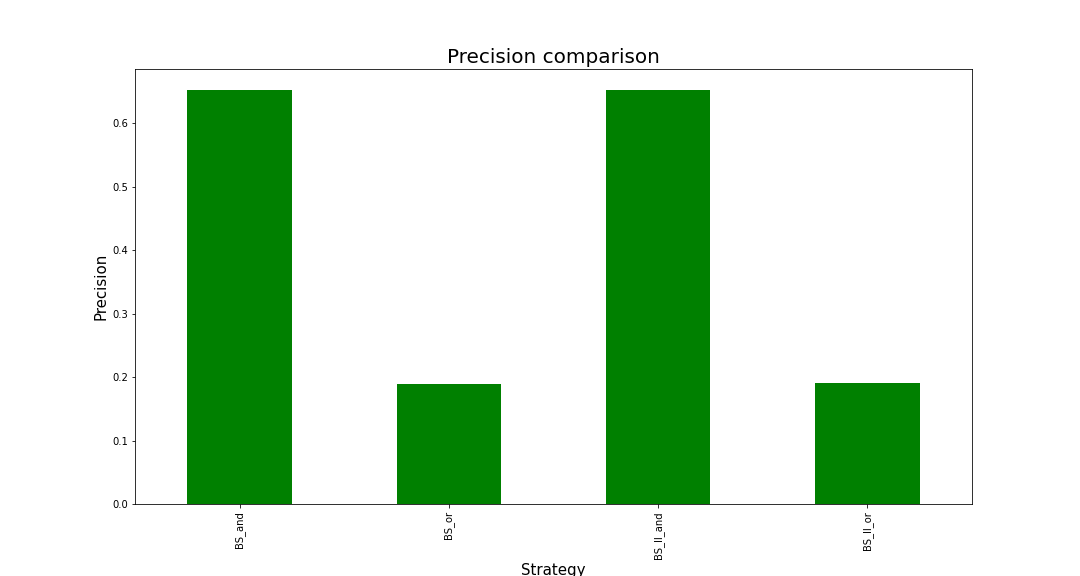
\includegraphics[width=\textwidth]{results/images/BS_precision_comparison.png}
    \caption{Precisión de cada estrategia.}
    \label{fig:Precision}
\end{figure}

El \textit{recall} (véase figura \ref{fig:Recall}), por su parte evalúa qué porcentaje de los documentos relevantes fueron recuperados. Con esto en mente, se espera que el resultado de esta métrica con las estrategias de disyunción sea muy buena, mientras que en las estrategias de conjunción resulta mala. Esto se debe a que existe la posibilidad de que un documento que no contiene todos los términos de la búsqueda sea relevante, por ejemplos sinónimos. Esto ocasiona que la estrategia de conjunción devuelva un valor mucho menor, pues retorna un porcentaje bajo del total de documentos que debería retornar.\\

\begin{figure}[H]
    \centering
    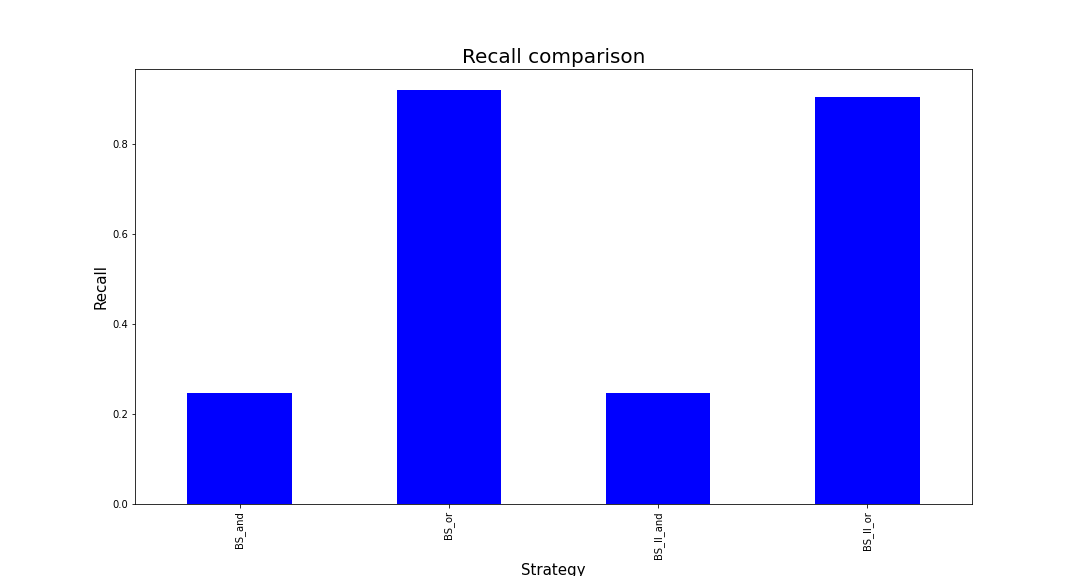
\includegraphics[width=\textwidth]{results/images/BS_recall_comparison.png}
    \caption{\textit{Recall} de cada estrategia.}
    \label{fig:Recall}
\end{figure}

Como se puede observar, las gráficas anteriores evidencian que bajo una de la luz de la métrica de precisión, las estrategias de AND retornan valores muchísimo más altos que los de OR, mientras que para \textit{recall} el resultado de las estrategias disyuntivas son muchísimo mejores. Es por esto que se recurre a una métrica que permita ponderar el resultado de precisión y \textit{recall}. F1-score (véase figura \ref{fig:F1-score}) es una métrica que pondera estos resultados. Se calcula como se muestra en la ecuación \ref{eq:recall}. 

\begin{equation}
    R = \frac{2PR}{P+R}
    \label{eq:recall}
\end{equation}

El resultado es ideal cuando es 1, pues significa que ambas métricas son perfectas. No obstante, es difícil de obtener. El resultado obtenido con las implementaciones actuales indica que el desempeño de las estrategias AND es mejor que el de las OR. Sin embargo, puede resultar conveniente ponderar de manera diferente el peso dado a cada métrica, en caso tal que resulte preferible obtener más documentos relacionados y no únicamente de los que se tenga total certeza de que son relevantes.

\begin{figure}[H]
    \centering
    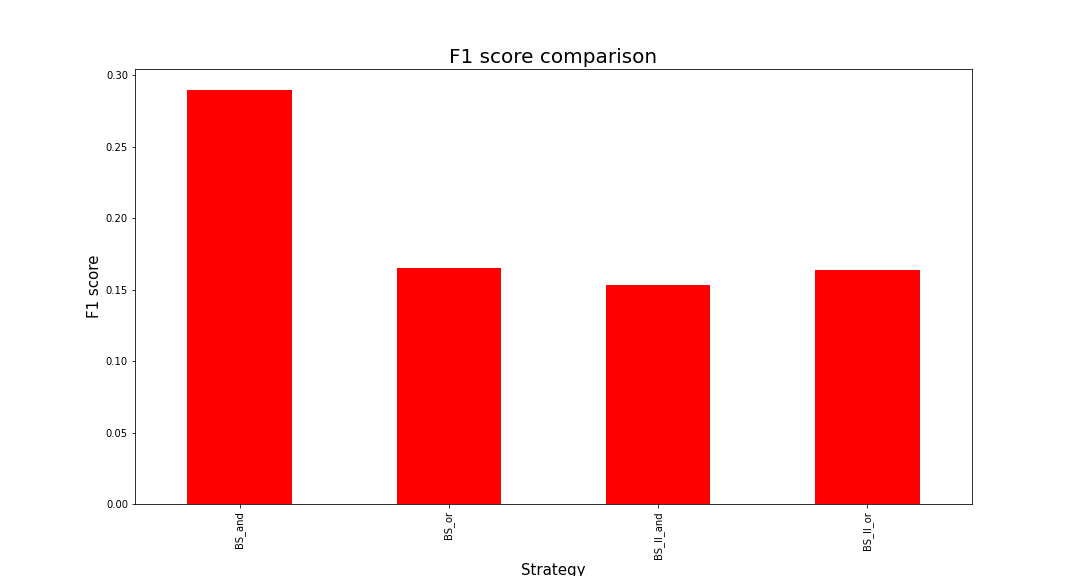
\includegraphics[width=\textwidth]{results/images/BS_f1_comparison.png}
    \caption{F1-score de cada estrategia.}
    \label{fig:F1-score}
\end{figure}

Finalmente, se destaca que los resultados de búsqueda binaria normal y búsqueda binaria con índice invertido son los mismos (para AND y para OR). La única diferencia está en el tiempo de ejecución de cada una, pues el índice invertido da mucha resulta mucho más eficiente. Los tiempos de ejecución para cada estrategia fueron:

\begin{itemize}
    \item \textbf{BS\_OR:} 1.315 s
    \item \textbf{BS\_AND:} 1.289 s
    \item \textbf{BSII\_OR:} 0.00497 s
    \item \textbf{BS\_AND:} 0.00185 s
\end{itemize}

Como es de esperarse, la estrategia de búsqueda binaria con índice invertido es mucho más rápida que la búsqueda binaria con el índice sin invertir. Esto se debe a que en vez de operar con una matriz sobre la cual se debe buscar en qué documento se presenta un término, el índice invertido puede identificar los documentos relevantes directamente a partir del término. 

Teniendo en cuenta las dos estrategias de búsqueda binaria analizadas con sus dos posibles operadores binarios se estableció que hay cuatro términos en los que la búsqueda que requiere el mayor consumo computacional cuando se hacen con la búsqueda binaria. Estas búsquedas corresponden a: \textit{q18}, \textit{q27}, \textit{q40} y \textit{q42}. Las cuatro búsquedas indicadas anteriormente pueden ser consideradas las más caras dado que son las que más términos tienen para la búsqueda. Por otra parte, se considera que la búsqueda binaria es la estrategia con mayor consumo computacional dado que debe recorrer una matriz de tamaño fijo en todas las búsquedas. Sin embargo, no hay una distinción del operador binario que sea utilizado porque la intersección de dos arreglos de tamaño fijo consume los mismos recursos sin importar qué operación binaria se lleve a cabo.

En caso tal que el número de documentos relevantes aumente se presentarían un aumento de costo computacional para las dos estrategias, solo que con condiciones diferentes. Por una parte, la búsqueda binaria debe recorrer todas las posiciones de una matriz por lo que si el tamaño de esta aumenta, el recorrido también lo hará. En este orden de ideas, el consumo computacional para la búsqueda binaria aumentará inevitablemente. Por otra parte, en el caso del índice invertido el aumento del consumo computacional se hará en la medida que los nuevos documentos sean relevantes para los términos. En este caso se podría dar la situación en la que una consulta utiliza términos que no son incluidos en los nuevos documentos, por lo que el consumo computacional para dicha consulta no aumentará. Sin embargo, lo más probable es que los nuevos documentos aumenten la cardinalidad de las listas de posteo, lo cual aumenta a su vez el consumo computacional y el tiempo de respuesta del sistema.

\begin{table}[h]
    \centering
    \begin{tabular}{|c|c|c|c|}
        \textbf{Estrategia} & \textbf{x100} & \textbf{x1000} & \textbf{x10000} \\
        BS\_OR & 131.5 & 1315 & 13150 \\
        BS\_AND & 128.9 & 1289 & 12890 \\
        BSII\_OR & 0.01491 & 0.01988 & 0.02485 \\
        BSII\_AND & 0.00555 & 0.0074 & 0.00925 \\
    \end{tabular}
    \caption{Estimación de tiempos de ejecución para las consultas con un aumento del tamaño de la colección.}
    \label{tab:estimations}
\end{table}

A partir de los tiempos de ejecución presentados previamente, la tabla \ref{tab:estimations} estima nuevos tiempos en función del número de veces en que aumente el tamaño de la colección. Se tiene que un aumento en la búsqueda binaria implicaría que se deben analizar más documentos en la matriz que compone el índice. En este orden de ideas, se espera que haya un aumento lineal del tiempo de ejecución para esta estrategia. En el caso del índice invertido, se tiene que un aumento de la colección no implica un aumento en las listas de posteo. Sin embargo, se espera que estas aumenten de tamaño aunque no de forma lineal. Para modelar un aumento de estas, lo cual va a afectar el tiempo de ejecución, se incluye un aumento en un factor logarítmico. 

Para incluir nuevos documentos en el índice de una búsqueda binaria se deben ejecutar los siguientes pasos:

\begin{enumerate}
    \item Agregar filas al índice con el fin de asociarlos a los nuevos documentos.
    \item Llenar las filas de los nuevos documentos con unos o ceros dependiendo de la presencia o no, respectivamente, de los términos en dichos documentos.
\end{enumerate}

Vale la pena mencionar que en caso tal que los documentos nuevos contengan un vocabulario considerablemente diferente al actual, será necesario agregar columnas al índice para considera los nuevos términos. Será necesario recorrer toda la colección con el fin de incluir los términos a los documentos antiguos en caso de ser necesario. Cuando se agregan nuevos documentos a un índice invertido es necesario realizar las siguientes acciones:

\begin{enumerate}
    \item Organizar los términos presentes en los nuevos documentos con un criterio lexicográfico.
    \item Iterar sobre los documentos que van a ser agregados.
    \item Para cada término de un documento, ir agregando el identificador a la lista de posteo correspondiente.
\end{enumerate}

En caso tal que se deba agregar vocabulario al índice invertido es necesario incluir el término según el ordenamiento lexicográfico. De igual manera, se deben recorrer todos los documentos de la colección con el fin de garantizar que el índice invertido es construido apropiadamente.

\subsection{Comparación de estrategias clasificadas (\textit{ranked}): RRI, RRDV, GENSIM}

Para evaluar el desempeño de las estrategias de recuperación de la información clasificadas \textit{(ranked)}, se realizó el calculo de las métricas \texttt{P@M}, \texttt{R@M}, \texttt{NDGC@M} y \texttt{MAP} para cada uno de los 35 \textit{queries} en el dataset, donde $M$ representa el número de documentos relevantes en la etiqueta. Para esto se hizo uso de las funciones desarrolladas en la primera parte de este trabajo, las cuales se encuentran en el archivo \texttt{metrics.py}. Como resultado de este proceso se obtuvieron las figuras \ref{fig:rankedP} - \ref{fig:rankedNDCG} y el cuadro \ref{tab:rankedResults} que resume los resultados promedio de todas las estrategias implementadas. \\

En términos generales, se puede observar que los resultados de todas las estrategias \textit{ranked} son bastante buenos. Salvo en dos ocasiones, todas las estrategias son capaces de recuperar al menos un documento relevante para el \textit{dataset} de 35 \textit{queries}. De igual forma, en varios casos se obtienen valores de \textit{precisión}, \textit{recall} y de \textit{NDGC} de 1, lo que representa una recuperación perfecta (se retronaron todos los documentos relevantes en el orden correcto). Vale la pena aclarar que en la mayoría de los casos el resultado de las estrategias de IR, recuperaba muchos más documentos de los que el archivo de etiquetas sugería como relevantes. No obstante, al estar estos resultados ordenados y al hacer la evaluación del desempeño hasta M (salvo por el MAP), se obtiene un desempeño adecuado. 

\begin{figure}[H]
    \centering
    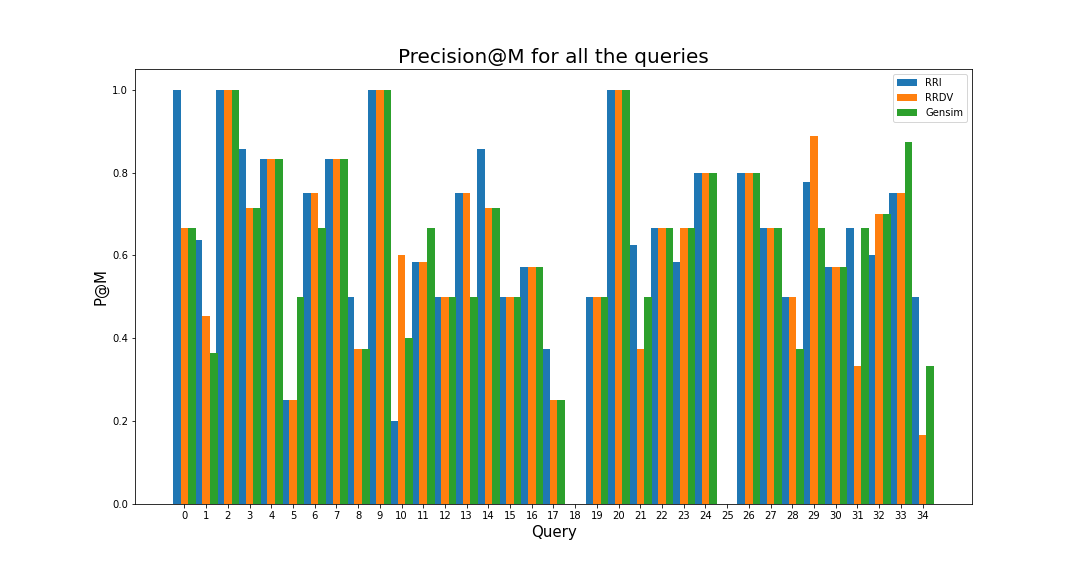
\includegraphics[width=\textwidth]{doc/images/P@M_Ranked.png}
    \caption{Resultados de P@M para todas las \textit{queries} del data set con las estrategias clasificadas (\textit{ranked})}
    \label{fig:rankedP}
\end{figure}

\begin{figure}[H]
    \centering
    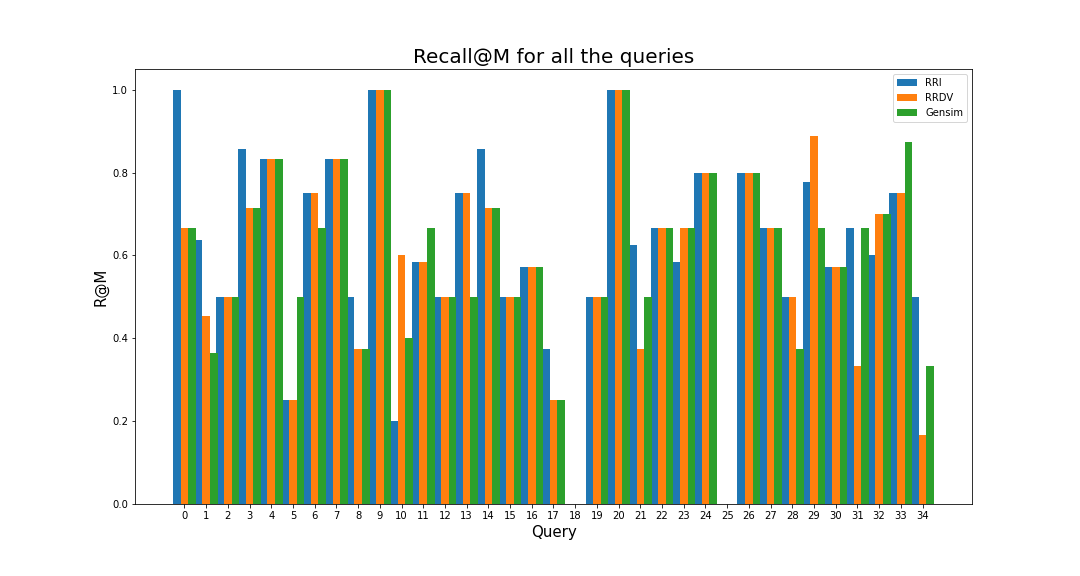
\includegraphics[width=\textwidth]{doc/images/R@M_Ranked.png}
    \caption{Resultados de R@M para todas las \textit{queries} del data set con las estrategias clasificadas (\textit{ranked})}
    \label{fig:rankedR}
\end{figure}


\begin{figure}[H]
    \centering
    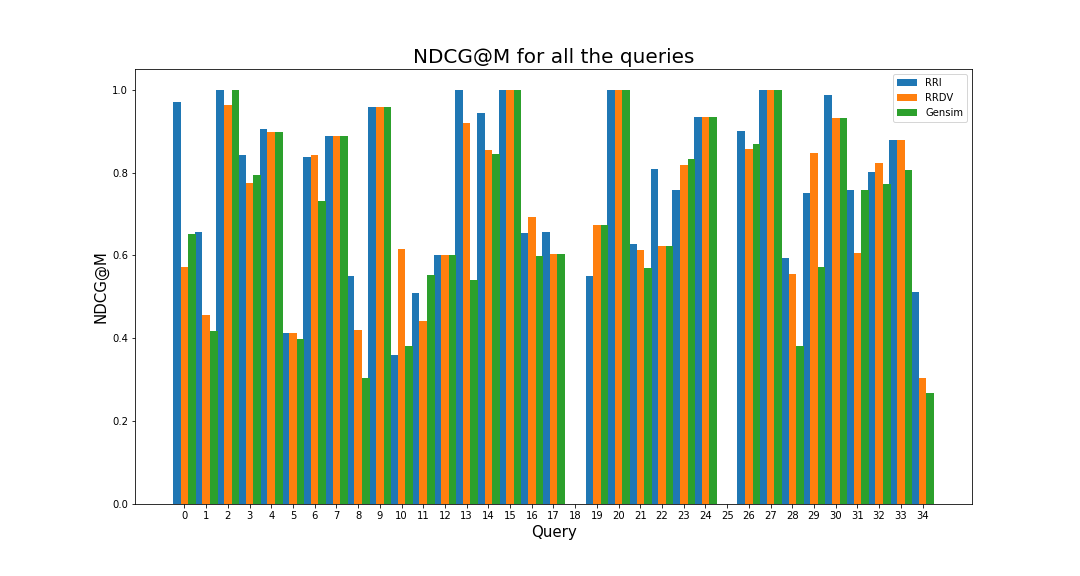
\includegraphics[width=\textwidth]{doc/images/NDCG@M_Ranked.png}
    \caption{Resultados de NDCG@M para todas las \textit{queries} del data set con las estrategias clasificadas (\textit{ranked})}
    \label{fig:rankedNDCG}
\end{figure}

Al momento de comparar el desempeños de las estrategias, se puede observar que, en promedio, RRI presenta mejores resultados que RRDV y Gensim en todas las métricas. Aunque en general los resultados de las 3 estrategias son bastante comparables y sus resultados no difieren en mucho. Adicionalmente, se puede observar que RRDV y Gensim tienen desempeños aun más cercanos, en cuanto a la precisión estos son casi iguales, en cuanto al Recall Gensim es ligeramente mejor y en cuanto al NDCG y al MAP la implementación de RRDV es mejor. \\

Se podría pensar que al aplicar la misma estrategia sobre el mismo \textit{dataset} los resultados deberían ser los mismos. No obstante, existen distintas variaciones que se le pueden aplicar a esta estrategia, la cual cambia sus resultados. Para este caso en especifico, la librería de Gensim, muestra en su documentación distintas formas de pesar las medidas de $tf$, $df$ y realizar la normalización de documentos. Al utilizar la configuración por defecto, se toma como medida de $tf$ el conteo crudo \textit{(raw frequency)} de los términos en el documento, el $idf$ y una normalización de documentos con similaridad coseno. Por su parte la implementación de RRDV realizada es muy similar, pero incorpora un peso logarítmico sobre el $tf$ (véase ecuación \ref{eq:tfidf}). Así las cosas, se podría decir que el efecto de suavizar la frecuencia del $tf$ con la función logaritmo, brinda un beneficio en cuanto al orden de los documentos, pues se obtiene un NDGC@M y un MAP significativamente mayores; pero con una ligera reducción en el desempeño del \textit{Recall} y una precisión prácticamente igual.

\begin{table}[H]
\centering
\begin{tabular}{|l|c|c|c|c|}
\hline
\textbf{Estrategia} & \multicolumn{1}{l|}{\textbf{Mean P@M}} & \multicolumn{1}{l|}{\textbf{Mean R@M}} & \multicolumn{1}{l|}{\textbf{Mean NDCG@M}} & \multicolumn{1}{l|}{\textbf{MAP}} \\ \hline
\textbf{RRI} & 0.6287 & 0.6144 & 0.7317 & 0.7340 \\ \hline
\textbf{RRDV} & 0.5923 & 0.5780 & 0.6967 & 0.6972 \\ \hline
\textbf{Gensim} & 0.5955 & 0.5812 & 0.6618 & 0.6592 \\ \hline
\end{tabular}
\caption{Resumen de resultados de desempeño para las estrategias clasificadas (\textit{ranked}).}
\label{tab:rankedResults}
\end{table}

Ahora bien, además de su desempeño, las estrategias de RRI y RRDV tienen otras diferencias que vale la pena mencionar. Por un lado, RRDV hace uso del concepto de documentos como vectores, en donde tanto el corpus de documentos, como los \textit{queries} (y en general cualquier agrupación de palabras) son tratados como vectores de un modelo de bolsa de palabras (BOW Model). Por el otro lado, RRI utiliza los pesos de \textit{tf-idf} para comparar puntajes (\textit{scores}) entre documentos a partir de un \textit{query}. Con esto en mente, el enfoque que propone RRDV puede ser ventajoso por su flexibilidad, pues se puede hacer una comparación de similaridad entre cualquier texto. En este caso, los \textit{queries} y en los documentos se piensan todos en un mismo espacio vectorial, con todas las ventajas que eso conlleva: como la capacidad de crear normas y distancias especificas para la tarea deseada. \\

No obstante, en términos de costo computacional, el enfoque de RRDV parece ser el más costoso. Esto se debe a que típicamente los modelos de bolsa de palabras (BOW) tienen vectores con una alta dimensionalidad (tamaño del vocabulario) y son muy dispersos. Adicionalmente, para realizar la tarea de IR se debe completar un paso adicional de similaridad, el cual conlleva a realizar un producto punto entre dos vectores de este tipo. Al contrastar esto con el enfoque de RRI, en donde solo se debe hacer la suma de los pesos de \textit{tf-idf} (valores ya guardados) sobre los distintos términos del \textit{query}, los cuales además tienden a ser pocos, da una idea de porque este enfoque puede ser mucho más eficiente. \\

A nivel empírico este razonamiento concuerda con las implementaciones realizadas y se podría probar de forma experimental. Sin embargo, y aunque se cumple de forma evidente en las estrategias implementadas desde cero, el desempeño de Gensim es bastante eficiente. Esto lleva a pensar que existen muchas formas de mejorar la implementación en cuanto a costo computacional y también a que existe un gran número de factores que pueden alterar dicha eficiencia, como el tamaño del vocabulario, el tamaño de los \textit{queries}, el tamaño de los documentos, entre otras cosas. \\

Finalmente, en el caso de que 100 nuevos documentos se incorporen a la colección los cambios requeridos pueden llegar a ser ligeramente distintos a los de una búsqueda binaria. Además del respectivo procesamiento inicial que requiere cada uno de los nuevos documentos (véase figura \ref{fig:preprocess}) es necesario tener en cuenta algunos detalles adicionales. Por un lado, no basta con agregar los documentos bien sea a la matriz de pesos de \textit{tf-idf} o al índice invertido que guarda el $tf$, sino que es necesario recalcular el $df$ de cada uno de los términos, pues el número de documentos en los que ahora aparece cada termino puede aumentar. No obstante, el $tf$ no será algo que requiera ser recalculado, pues esta medida depende únicamente de cada documento, y solo deberá ser calculada para los nuevos documentos. Ahora bien, esto sería bajo el supuesto de que el vocabulario actual (de alrededor de 18000 palabras para el \textit{dataset} en cuestión) sirva para los 100 nuevos documentos. En caso de que estos nuevos documentos fueran de un dominio totalmente distinto, y el vocabulario actual no respondiera a esto, sería necesario volver a construir el vocabulario y realizar nuevamente todo el proceso para la construcción de las estrategias de IR.


\newpage
\bibliographystyle{unsrt}
\bibliography{biblist.bib}

\end{document}